
%
% File: chap03.tex
% Author: Antigoni Kourou
% Description: The proposed approach
%
\let\textcircled=\pgftextcircled
\chapter{The proposed approach}

\label{chap:prop}

\initial{F}or transforming the text feedback into quantitative data, which will serve as input for analysis purposes, this paper proposes an approach as shown in Figure \ref{fig:pipe}. The pipeline consists of four main steps: \textit{pre-processing, feature identification, sentiment detection}  and \textit{data analysis}. Initially, the whole input of the pipeline is the huge corpus of text reviews stored in Neo4J database. This big amount of data from social is considered to be very noisy, therefore it will be cleaned up as be described in the following section. Features and sentiment are then identified in text based in sentence level. The output of these three stages consists of the quantitative sentiment scores for sentences of reviews and the features identified in them. This output will then serve as the input data of the final stage of the pipeline: data analysis.  
The whole pipeline is built using Python programming language and its related packages. All the data analysis and visualization are written in Jupyter notebook. The following sections will explain each step of the proposed approach in further details.
%
%
%
\section{Pre-processing}
%
% -------------------------------------
% POS Tagging missing
% ------------------------------------0
The pipeline reads the text data from cloud with the help of \textit{py2neo}, a toolkit for working with Neo4J from within Python applications, and it formulates the queries in Cypher, the querying language for Neo4J graph database. The reviews in the corpus are read one by one and each of them is checked if it fulfills the language requirements. In my work, the whole concept of the pipeline is developed in English, as the most used language in e-tourism websites and as the easiest language for text mining. Thus, every time that the algorithm runs into a review not in English, it will ignore the review and continue with the next one. For each English review detected, the algorithm will cut the text into sentences, 
\begin{figure}[h!]
	\centering
	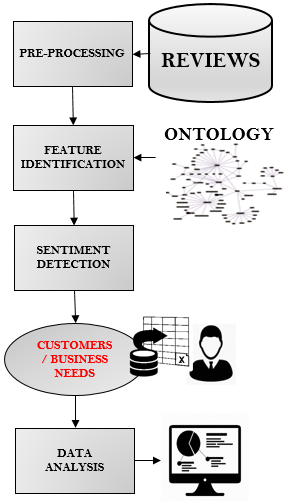
\includegraphics[height=0.5\textheight]{pipe}
	\caption{The proposed approach}
	\label{fig:pipe}
\end{figure} 
with the intention of detecting the sentiment in sentence-level and extracting features within these sentences. 
%
Afterwards tokenization and lemmatization are performed to each sentence of the review. Tokenization is used form chopping the sentences into words, phrases, symbols and emoticons, each represented as a token. Lemmatization is the process of getting the root of the words, called lemmas, while ignoring its other forms as part of the speech. For tokenization the pipeline uses the \textit{TweetTokenizer}\footnote{http://www.nltk.org/api/nltk.tokenize.html} package, part of NLTK and Twitter-aware designed, in order to be able to identify emoticons and adapt to new domains. On the other hand lemmatization is performed using \textit{WordNet}\footnote{https://wordnet.princeton.edu/}, a large lexical database for English terms, in which nouns, verbs, adjectives and adverbs are grouped into sets of cognitive synonyms (synsets), each expressing a distinct concept \cite{miller1995wordnet}. The output of these two steps is a list of lemmas for each sentence, which will be used by the next step in the pipeline as explained in the following section.  
%
\section{Feature identification}
As soon as each sentence in the corpus of reviews is represented as a list of lemmas, an ontology based approach is used to identify the accommodation features of each sentence. The ontology is chosen for feature identification as a way for detecting all the terms, concepts and relations linked to accommodation domain. Prior to identifying the features, the pipeline builds a list of synonyms, hyponyms and hypernyms for every term of the ontology, in order to increase the range of matches found in the text. The list is based on the Synsets and relations between concepts as introduced by WordNet library. The lists of related terms is lemmatized, as explained above, and the duplicates are removed. The lemmatization process aims to create a list of related lemmas for each feature in the ontology, which would then be used for feature identification in the sentences.
Thus, the feature identification steps is a string match of the list of lemmas for every single sentence, with the list of related lemmas of every feature in the ontology. Considering that the ontology consists of many terms, this sample pipeline is trained to identify only six features that Airbnb asks the customers to manually rate as part of their feedback, namely \textit{accuracy, cleanliness, check-in, communication, location} and \textit{value}. However, the conclusion are drawn equally as all the features of ontology are included.
When a word in the sentence is identified to be a feature, the algorithm jumps to the next word of the sentence. Within one sentence more than one feature can be identified, as well as features can be mentioned more than once. Therefore, for every possible feature match, a\textit{ match counter } variable which keeps track of the features mentioned is assigned to the sentence. Here, the pipeline considers each sentence as independent and it ignores the logical connection between two sentences of the same review.

\section{Sentiment detection}
A very important part of the pipeline is sentiment detection. The algorithm used for this purpose is VADER (Valence Aware Dictionary for Sentiment Reasoning) \footnote{https://pypi.python.org/pypi/vaderSentiment}, part of Python packages. VADER is a lexicon and rule-based sentiment analysis tool that is specifically attuned to sentiments expressed in social media. For building the valence scores for sentiment intensity, VADER considers several well-known sources, such as ANEW, SentiWordNet and SenticNet. These dictionaries include not only lexical features, but also grammatical and syntactical rules.
Therefore, VADER is able to deal with negation, capital letters, degree modifiers, emoticons, punctuation types, contrastive conjunctions (\textit{but, however}and slangs.  Based on the comparisons of 22 sentiment mining tools of the last decade, VADER is ranked as the best algorithm for comments and the second best for social networks \cite{ribeiro2015benchmark}. Some of its assigned scores are \textit{(good 0.7); (great 0.9434); (awesome	0.8306); (dirty -0.83066); (terrible -0.9434)} \footnote{The full lexicon can be found in: https:\/\/github.com\/cjhutto\/vaderSentiment\/tree\/master\/additional\_resources}. In this paper, the pipeline uses VADER to return a sentiment score for every sentence of the review, which would afterwards serve as a discrete score for the identified features in that sentence. Considering that in one sentence, more than 1 feature can be identified or the same feature can be identified more than once as mentioned above, a probabilistic model is developed. This model serves for defining the probabilities that a sentiment score would reflect user's opinion on each explicit feature identified within one sentence. 

The dataset consists of 2 356 listings, \textit{L = \{ L\textsubscript{0}, L\textsubscript{1},  L\textsubscript{2} ... L\textsubscript{2355} \}}. Each listing in this corpus can be represented by the ID of the listing in the database \textit{lis\_id}. Every listing from this set has a number of reviews, which varies from one listing to the other and is identified from ID of the review \textit{R\textsubscript{lis\_id} = \{ R\textsubscript{0}, R\textsubscript{1},  R\textsubscript{2} ... R\textsubscript{r} \}}. For a single review of a certain listing would be \textit{R\textsubscript{lis\_id, rev\_id}}. This review is composed by a number of sentences \textit{S\textsubscript{lis\_id, rev\_id} = \{S\textsubscript{0}, S\textsubscript{1}, S\textsubscript{2} ... S\textsubscript{s}\}}. 
The pipeline is trained to detect the sentiment of all the sentences, which will be in the same form as the one above. 
In each of these sentences, the pipeline is trained to identify six accommodation features \textit{F = \{accuracy, check-in, cleanliness, communication, location, value\}}. When the sentiment of a sentence is detected, it does not particularly refer to a certain feature. In order to calculate the part of the sentiment that belongs to a certain feature identified in the sentence, we use a probabilistic model. According to this model, the probability that the compound sentiment score refers to a certain feature is p\textsubscript{i}, where \textit{i} is the index of the feature from the list F. This probability is uniformly distributed between the identified features and is calculated as 1/k, where \textit{k} is the number of features mentioned. Likewise, if the feature is not identified in the sentence the probability would be 0.
%
% ----------------FORMULA---------------------
$$Sentiment = \sum_{i=1}^{n}p\textsubscript{i} *  sentiment\textsubscript{ i} \hspace{1cm} (1)$$ 
%---------------------------------------------
%
This formula for calculating the sentiment of the features is part of the sentiment detection phase of the pipeline and it is repeated for every single sentence. For instance, considering the reviews of listing 24328,  \textit{R\textsubscript{24328, 10146}} would represent the review: "We had a great stay at Joe's. The handy guide to the house and neighborhood was much appreciated, as were Joe's clear instructions for checking in while he was away. The house was comfortable and eclectic, full of personal character." Thus, \textit{S\textsubscript{24328, 10146, 1}} represents the second sentence of the text above. In this sentence can be identified three features \textit{check-in, communication,} and \textit{location}. The compound sentiment score of the sentence above has in this way to refer to one of these features in a probability of 33.3\%. Figure \ref{fig:sent} shows the results of the pipeline for this case. 
\begin{figure}[h!]
	\centering
	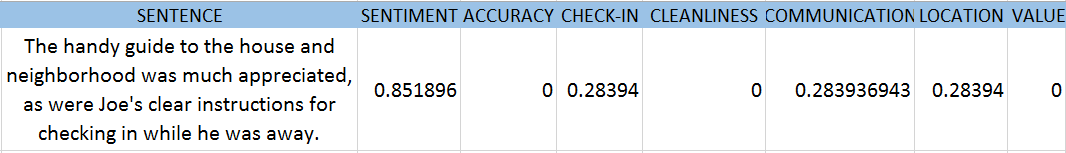
\includegraphics[height=0.1\textheight]{example_pip}
	\caption{Example of the probabilistic sentiment results}
	\label{fig:sent}
\end{figure}

%

\section{Data analysis}
% 
% will explain the analysis process using Pandas for different cases! 
%
The last step of the pipeline and the most interesting one for service providers and businesses is data analysis. Up to here, we saw the pipeline processing all the text data step by step and transform it into meaningful sentiment scores for each sentence and each accommodation feature of the reviews. The output of these phases is a Comma Separated Vector (.csv) file, consisting of all listings, all listings' reviews, its respective sentences and the sentiment for the identified features on these sentences. This scores are analyzed with Pandas\footnote{http://pandas.pydata.org/}, an open source library providing high-performance, easy-to-use data structures and data analysis tools for the Python. The workspace  of analysis and visualization of results is Jupyter Notebook, a web application that allows users to create and share documents that contain  interactive code, equations, visualizations and explanatory text. The data  analysis in this step includes calculation and visualization of sentiment scores per reviews and listings, frequency of ontology-based features, ranking of listings based on overall sentiment or based on sentiment of one or more specific features, ranking of features for one listing based on their sentiment, identification of listings with the biggest number of reviews and identification on listings where the host have canceled once or more the reservation, computation and comparisons of sentiment scores from the pipeline with the ratings of Airbnb and so further. An example of the analysis, Figure \ref{fig:comp} shows all the listings with low rating (less than 4 stars since the lowest rating is 3 stars) and visualizes the differences between the sentiment scores generated from the pipeline and the ratings found on Airbnb.  The analysis can of course be extended and customized to match the specific interest of the service providers or the customers. The main results of this analysis with be explored in the results section, followed by the implementation of pipeline according to its usefulness for service providers and customers respectively. 
\begin{figure}[h!]
\centering
	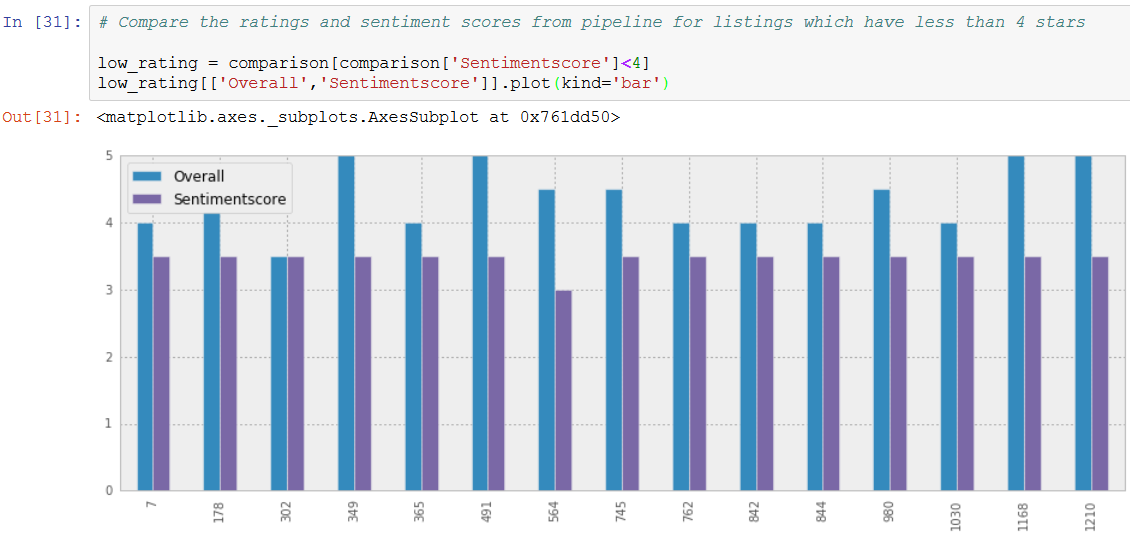
\includegraphics[height=0.25\textheight]{data_comparison}
	\caption{Example of data analysis in Jupyter Notebook with IPython \& Pandas Library}
	\label{fig:comp}
\end{figure}
